\chapter{Soft Brownian Offset}

Soft Brownian Offset (SBO) è un algoritmo per la generazione di dati sintetici fuori dalla distribuzione (Out of Distribution OOD). 

È stato sviluppato da ~\cite{sbo} inizialmente per poter migliorare il rilevamento dei dati fuori dalla distribuzione, si pensi ad esempio nel caso dei cyber-physical systems (CPS) e.g. auto a guida autonoma, dove il rilevamento di eventi anomali è di vitale importanza ~\cite{yuhasEmbeddedOutofdistributionDetection2021}.

Per questo scopo i dati generati necessitano di essere non troppo dissimili da quelli originali, perché altrimenti il modello potrebbe soffrire di ``overconfidence'' ~\cite{amodeiConcreteProblemsAI2016}.

SBO si basa sul ``Gaussian Hyperspheric Offset'' che cerca di creare i dati OOD campionando attraverso una ipersfera attorno ai dati iniziali nella distribuzione (In Distribution).

Partendo da quest'ultimo algoritmo, SBO permette di utilizzare qualsiasi punto del dataset e traslarlo in modo da avere una certa distanza minima dagli altri punti. I dati vengono processati da un autoencoder (AE) addestrato sul dataset di riferimento. La figura \ref{fig:sbo_schema} mostra graficamente questo approccio. 

Soft Browninan Offset è ispirato al moto browniano e traduce il concetto nella sua rappresentazione in $R^D$ usando le ipersfere.

In particolare, l'algoritmo cerca di traslare i punti iterativamente in modo da avere una distanza minima chiamata $d_{min}$ dal punto originale. All'aumentare del valore $d_{min}$ si aumenta quindi la distanza dei punti sintetici dai punti originali, questo lo si può notare dalla figura \ref{fig:sbo_dmin} dove è presente anche il parametro $softness$ utilizzato per regolare il riempimento delle aree vuote.


\begin{figure}[htpb]
    \centering
    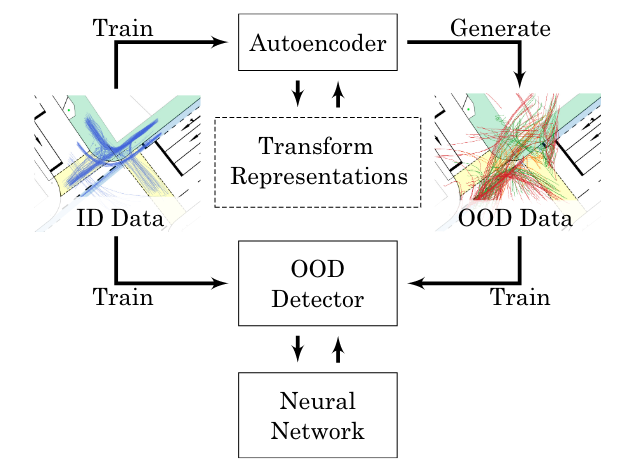
\includegraphics[width=\textwidth,height=10cm,keepaspectratio=true]{img/sbo_schema.png}
    \caption{
        Schema che rappresenta l'approccio utilizzato da SBO. Inizialmente i dati ID vengono usati per addestrare l'autoencoder e successivamente vengono generati i dati OOD tramite SBO. Questi poi vengono decodificati dall'AE per integrarsi nel dataset iniziale. Infine, viene addestrata una rete neurale, nel nostro caso invece, utilizzeremo XGBoost.
    }
    \label{fig:sbo_schema}
\end{figure}

\begin{figure}[htpb]
    \centering
    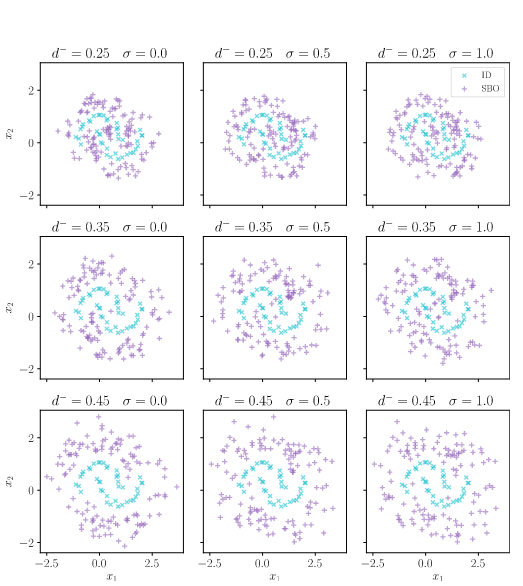
\includegraphics[width=\textwidth,height=10cm,keepaspectratio=true]{img/sbo_dmin.png}
    \caption{
      La figura rappresenta come si distribuiscono i dati sintetici (in lilla) rispetto ai dati originali (in azzurro) al variare del parametro $d_{min}$ e $softness$.
    }
    \label{fig:sbo_dmin}
\end{figure}


\section{Autoencoder} 

Un autoencoder è una particolare rete neurale che ha il compito di codificare un input e comprimerlo in una rappresentazione rilevante per poi decodificarlo e ricostruirlo nel modo più fedele possibile ~\cite{bankAutoencoders2021}.

Il loro compito principale è quindi di imparare, in modo non supervisionato, una rappresentazione ridotta significativa dei dati.

Il problema può essere formalmente definito ~\cite{baldiAutoencodersUnsupervisedLearning}, come trovare le funzioni $A$:$ R^{n} \rightarrow R^p$ (encoder) e $B$:$ R^{p} \rightarrow R^n$ (decoder) in modo che:

\begin{center}
$arg min_{A,B} E$[$\Delta$($x,  B$($A$($x$)))] \\
\end{center}

dove $E$ è la distribuzione di $x$ che ci si aspetta, e $\Delta$ è la funzione obbiettivo della ricostruzione, che misura la distanza tra l'output del decoder e l'input.

La figura \ref{fig:ae_schema} mostra il processo del modello autoencoder.

\begin{figure}[htpb]
    \centering
    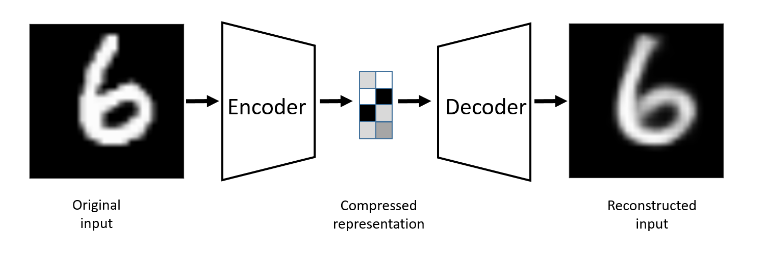
\includegraphics[width=\textwidth,height=10cm,keepaspectratio=true]{img/ae_schema.png}
    \caption{
        Schema che rappresenta il modello autoencoder. Da ~\cite{baldiAutoencodersUnsupervisedLearning}
    }
    \label{fig:ae_schema}
\end{figure}


L'approccio utilizzato per Soft Brownian Offset è quello di addestrare un autoencoder sul dataset di partenza, ridurre lo spazio di lavoro usando l'encoder, generare i dati OOD ed infine ricostruire il dataset attraverso il decoder.



